%TODO anonymize
%TODO remove all references
%TODO remove all we
%TODO Larger images
\documentclass{sig-alternate}

\usepackage{graphicx,url,natbib}
\usepackage[tight,footnotesize]{subfigure} 


%\usepackage{wallpaper}
\begin{document}

%\CenterWallPaper{1.0}{images/lightenedgray.png}

\conferenceinfo{GECCO'11,} {July 12--16, 2011, Dublin, Ireland.}
\CopyrightYear{2011}
\crdata{978-1-4503-0690-4/11/07}
\clubpenalty=10000
\widowpenalty = 10000

\numberofauthors{7}
\title{Meta Pylons}
\author{
% 1st. author
% Jonathan Byrne\\
% \alignauthor
% Michael Fenton\\
% \alignauthor
% Erik Hemberg\\
% \alignauthor
% Elizabeth Shotton\\
% \and
% Ciaran McNally\\
% \alignauthor
% James McDermott\\
% \alignauthor
% Michael O'Neill\\
}

\maketitle

%Assessment Criteria
%Stage One
%Design Quality (40%)
%- appearance
%- creative response
%- quality and clarity of presentation
%Response to and understanding of Brief (40%)
%- construction approach
%- technical viability
%- functionality and practicality
%Philosophy and Approach (20%)
%- design philosophy


%Philosophy and Approach (20%)
%- design philosophy

The natural process of biological evolution has clearly demonstrated
its power to design elegant form and structure in the name of
survival. Therefore, it is natural to employ algorithms which are
inspired by this process to tackle design problems. These evolutionary
algorithms (EAs) are powerful problem-solving tools e.g. genetic
programming (GP) is now capable of routine human-competitive
performance in the area of analog circuit design~\cite{koza2003}.

Meta pylon is more then a design, it is a method which allows the
transformation of pylons in a natural way. Such a method is very
useful when tackling the challenges to the UK's energy infrastructure
where the target of an 80\% reduction in carbon emissions by 2050 in
the UK, means substantial change. In order to deliver electricity to
homes, communities and businesses, the UK will see a significant
increase in the number of pylons. The optimization process in the Meta
Pylon method aids in achieving this goal through minimization of the
pylon weight, thus minimizing the resources used.

We are using an EA based on a grammar, grammars allow a natural way to
encode human domain knowledge into the generative process, and are
proving invaluable in the area of generative
design~\cite{oneill2010}. The grammar geneartes the designs and the
software creates and selects new designs.

\section*{Design Philosophy - Evolutionary Algorithms}
By using EAs in the design the exploratory process is not limited or
biased by the imagination of the human user or preconceptions based on
prior typologies or known solutions. Thus designs which are novel and
sometimes counterintuitive can be produced. The evolutionary search
introduce an explicit bias in the form of architectural and
engineering domain knowledge. This can be achieved by allowing the
user to specify structural forms, planning constraints, and even
aesthetic preferences a priori. Finally, it is possible to allow the
designer to interactively select designs.

A basic pylon structure is modifed and validated against the
constraints in the specification, thereby creating a plethora of
varying designs. The volume, speed and novelty of which the designs
are generated and tested are impossible for the human designer to
achieve. Instead, the designer provides invalueable expert knowledge
and intelligence by filtering the designs. Thus achieving a
symbiotic man--machine relationship.

The idea of using the current pylon design as a base comes from the
observation that the existing pylons have almost blended into peoples
perception of the landscape, as well as being strucutarlly tested by
time. In addition to conserving traditions our approch adds more
diversity in the electrical pylon ecosystem and the ability to create
naturally bespoke pylons. Figure~\ref{fig:pylon_montage} shows the
wide variety of designs.

\begin{figure*}
\centering
  \includegraphics[width=0.96\textwidth]{images/TJMqPs.png}
  \caption{Electric Pylon Ecosystem}
  \label{fig:pylon_montage}
\end{figure*}

\section*{Evolutionary Design of Pylons}
%Design Quality (40%)
%- appearance
%- creative response

The software automatically generates pylons and evaluate them
according to the specifications using software. After the search for
pylons that optimally conform to the multiple constraints the myriad
of suggestions and pick the most aestetically pleasing is selected,
see Figure~\ref{fig:EA_general} for an overview of the evolutionary
design process. We first initialize a population, then evaluate it and
while no optimum has been found or max iterations has not been
reached: select individual solutions from the population, apply
operators to the selected solutions and replace the population.

\begin{figure}
\centering
  \includegraphics[width=0.46\textwidth]{images/EA_general}
  \caption{Flow of a canonical Evolutionary Algorithm. First
    initialize a population, then evaluate the population, while not
    optimum found or not max iterations reached: select individual
    solutions from the population, apply operators to the selected
    solutions and replace the population.}
  \label{fig:EA_general}
\end{figure}

An EA method called Grammatical Evolution~\cite{oneill2010} was
modified to generate the pylons. A template for the pylons is encoded
in the form of a grammar. Rules from the grammar are selected by the
EA to generate different types of pylons. Although the grammar only
consists of a limited number of rules, those rules may be called
repeatedly to generate highly complex objects, i.e.~there is a bounded
recursion in the grammar. The total number of pylon combinations that
can be created is quite large, approximately $5.918e+23$, which is
close to the number of grains of sands on earth. Although, all these
designs might not be feasible.

The structure of the pylon was generated procedurally. A generic
function was used to generate different sections of the pylon. To
create each level the section was called with parameters specific to
that section, such as arm width and cross-bracing type. Reusing the
same function meant that the pylon code was compact and generated
uniformity between the different sections.

Our grammar took advantage of fractals as a method for generating the
necessary complex designs for our pylons. We adapted the recursive
method of creating Sierpinski triangles. Sierpinski triangles are
fractals composed by taking an existing triangle and subdividing it to
create several smaller internal triangles, see
Figure~\ref{fig:sierpinsky_triangles}. Finally, more designs of model
pylons are shown in Figure~\ref{fig:2EsBS}.

\begin{figure}
  \centering
  \subfigure[Sierpinski] {
    \label{fig:sierpinski}
    
\includegraphics[width=0.46\textwidth]{images/sierpinski.pdf}
  }\hfil
  \subfigure[Varinski] {
    \label{fig:varinski}
    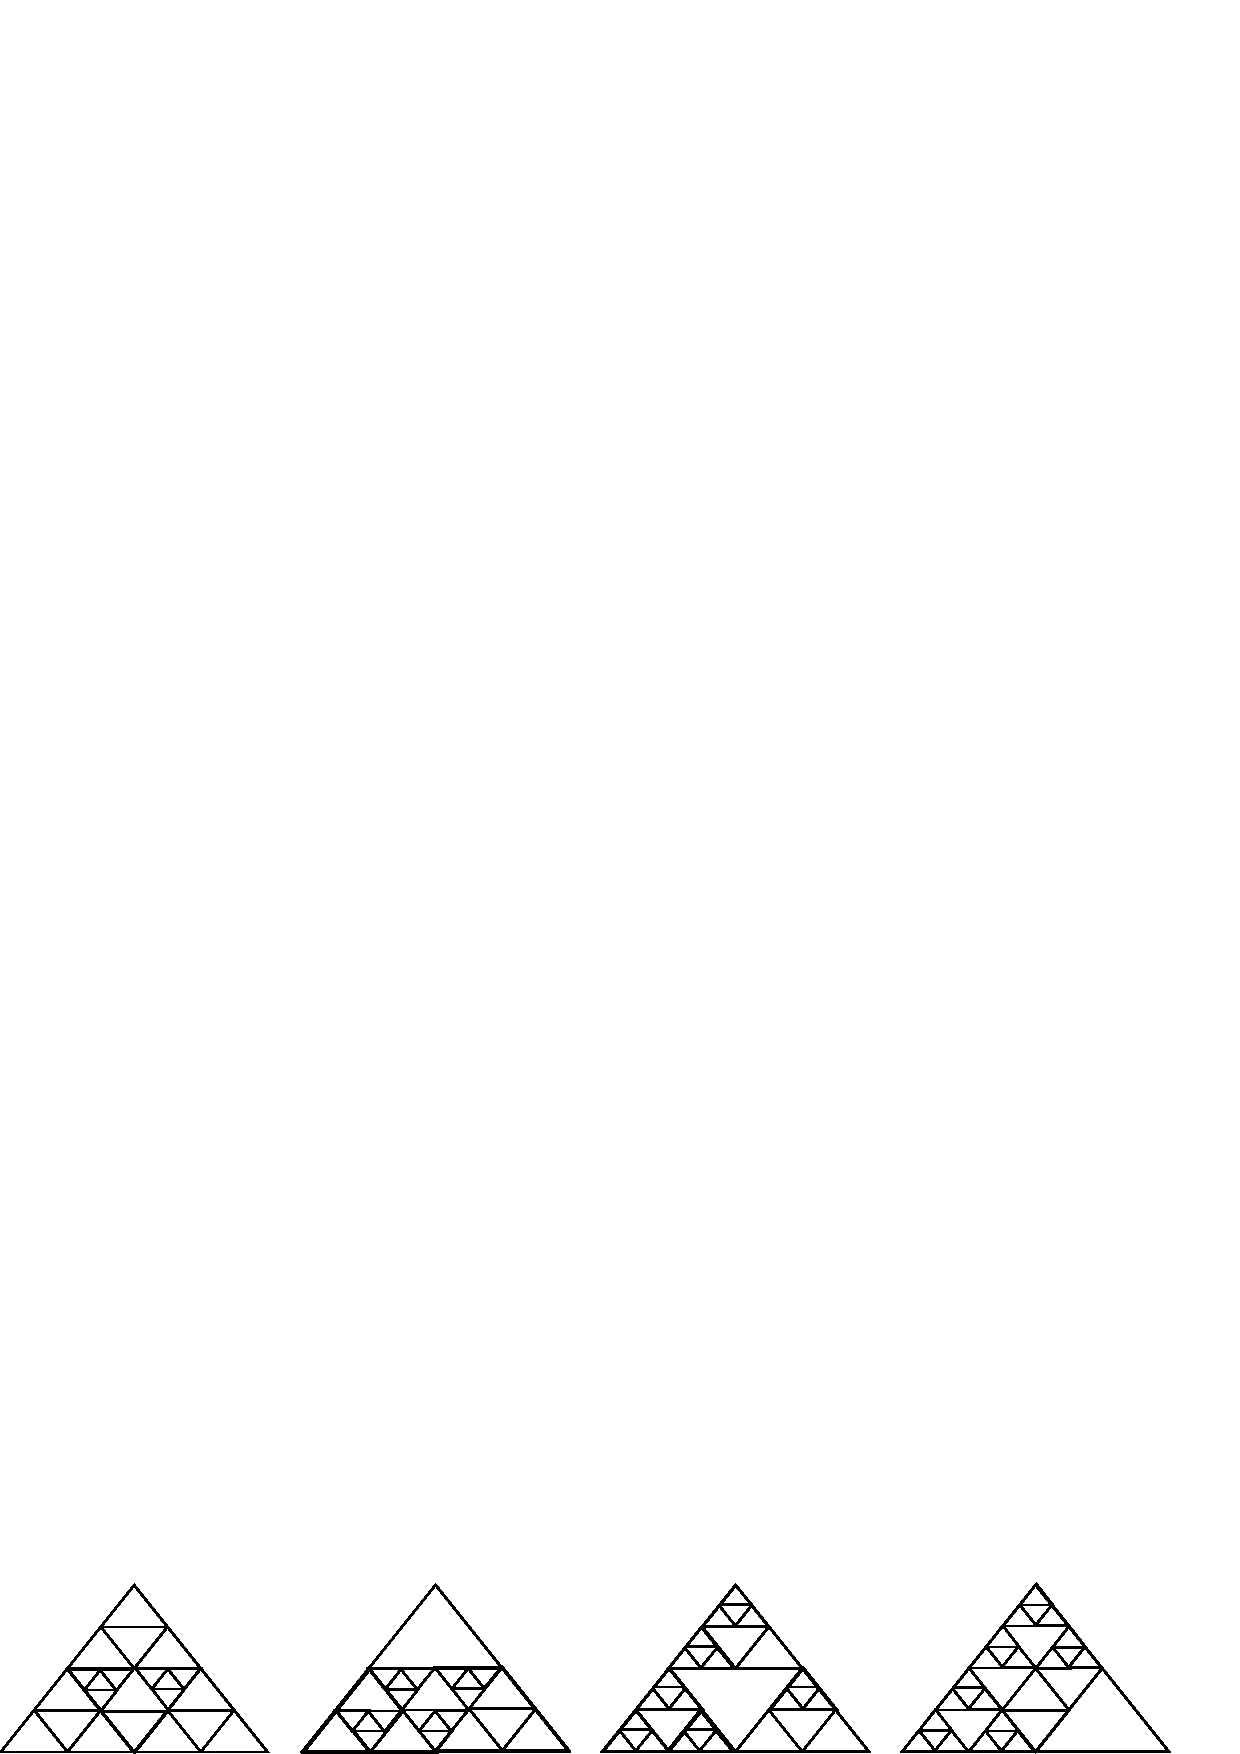
\includegraphics[width=0.46\textwidth]{images/varinski.pdf}
  }
  \caption{Sierpinsky triangles}
  \label{fig:sierpinsky_triangles}
\end{figure}

\begin{figure}
  \centering
  \subfigure[Pylon 1] {
    \label{fig:2EsBS}
    \includegraphics[width=0.46\textwidth]{images/2EsBS.jpg}
  }\hfil
  \subfigure[Pylon 2] {
    \label{fig:StortTorn1}
    \includegraphics[width=0.46\textwidth]{images/StortTorn1.jpg}
  }\hfil
  \caption{Model Pylons}
  \label{fig:pylons}
\end{figure}


\section*{Construction}
%Response to and understanding of Brief (40%)
%- construction approach
%- technical viability
%- functionality and practica

The fitness function is what determines the suitability of each
individual design for its particular role or roles in its
environment. We have modelled a physical environment by using a free
open-source finite-element analysis program called San Le's Free
Finite Element Analysis (SLFFEA)
(\url{http://slffea.sourceforge.net/index.html}. Using this software,
we can analyse each individual generated structure and then feed the
analysis data back into the main program, which allows us to
automatically evaluate the designs.

We use a multi-objective evolutionary optimization program that allows
for multiple objectives to be applied to the same
individual~\cite{fenton2011}. With this in mind, we included the
self-weight of the structure as a second goal to be minimized; this
ensured that lightweight yet low-stress structures are evolved, as the
two fitnesses are mutually opposing. The minimization of Compliance,
or Strain Energy. Being the inverse of the elasticity of the
structure, the less the compliance of a structure, the less likely its
tendency to deform will be (the stiffer it will
be)~\cite{Rozvany1998}. When this fitness was combined with the
minimization of overall structure deflections as a third fitness
objective, we obtained a trifecta of structural fitness functions: The
minimization of compliance, weight and observed deflection. This
ensures our search space is continually refined towards an optimal
pareto-front of solutions. Figures~\ref{fig:loaded_pylons_3},
\ref{fig:loaded_pylons_1} and \ref{fig:loaded_pylons_2} show the
different load cases, where 1 is without load, 2 is ? and 3 the
displacement.

Constant and variable list in the software.

\begin{figure}
  \centering
  \subfigure[Wind and ice load 1] {
    \label{fig:windIceload1}
    \includegraphics[width=0.2\textwidth]{images/stresses/windIceLoading1.png}
  }\hfil
  \subfigure[Wind and ice load 2] {
    \label{fig:windIceload2}
    \includegraphics[width=0.2\textwidth]{images/stresses/windIceLoading2.png}
  }\hfil
  \subfigure[Wind and ice load 3] {
    \label{fig:windIceload3}
    \includegraphics[width=0.2\textwidth]{images/stresses/windIceLoading3.png}
  }
  \caption{Loaded Model Pylons}
  \label{fig:loaded_pylons_3}
\end{figure}

\begin{figure}
  \centering
  \subfigure[Break load 1] {
    \label{fig:breakLoad1}
    \includegraphics[width=0.2\textwidth]{images/stresses/breakLoad1.png}
  }\hfil
  \subfigure[Break load 2] {
    \label{fig:breakLoad2}
    \includegraphics[width=0.2\textwidth]{images/stresses/breakLoad2.png}
  }\hfil
  \subfigure[Break load 3] {
    \label{fig:breakLoad3}
    \includegraphics[width=0.2\textwidth]{images/stresses/breakLoad3.png}
  }\hfil
  \subfigure[Ice load 1] {
    \label{fig:iceLoad1}
    \includegraphics[width=0.2\textwidth]{images/stresses/iceload1.png}
  }\hfil
  \subfigure[Ice load 2] {
    \label{fig:iceLoad2}
    \includegraphics[width=0.2\textwidth]{images/stresses/iceload2.png}
  }\hfil
  \subfigure[Ice load 3] {
    \label{fig:iceLoad3}
    \includegraphics[width=0.2\textwidth]{images/stresses/iceload3.png}
  }
  \caption{Loaded Model Pylons}
  \label{fig:loaded_pylons_1}
\end{figure}

\begin{figure}
  \centering
  \subfigure[Stress load 1] {
    \label{fig:stressLoad1}
    \includegraphics[width=0.2\textwidth]{images/stresses/stressLoad1.png}
  }\hfil
  \subfigure[Stress load 2] {
    \label{fig:stressLoad2}
    \includegraphics[width=0.2\textwidth]{images/stresses/stressLoad2.png}
  }\hfil
  \subfigure[Stress load 3] {
    \label{fig:stressLoad3}
    \includegraphics[width=0.2\textwidth]{images/stresses/stressLoad3.png}
  }\hfil
  \subfigure[Wind load 1] {
    \label{fig:windload1}
    \includegraphics[width=0.2\textwidth]{images/stresses/windload1.png}
  }\hfil
  \subfigure[Wind load 2] {
    \label{fig:windload2}
    \includegraphics[width=0.2\textwidth]{images/stresses/windload2.png}
  }\hfil
  \subfigure[Wind load 3] {
    \label{fig:windload3}
    \includegraphics[width=0.2\textwidth]{images/stresses/windload3.png}
  }
  \caption{Loaded Model Pylons}
  \label{fig:loaded_pylons_2}
\end{figure}

% \begin{flushleft}
% \bibliographystyle{abbrv}
% \begin{thebibliography}{17}
% \vspace*{0.5mm}
% {\scriptsize

% \providecommand{\natexlab}[1]{#1}
% \providecommand{\url}[1]{\texttt{#1}}
% \expandafter\ifx\csname urlstyle\endcsname\relax
% \providecommand{\doi}[1]{doi: #1}\else
% \providecommand{\doi}{doi: \begingroup \urlstyle{rm}\Url}\fi

% %TODO fix references
% \bibitem[Fenton et~al.(2011)]{fenton2011} 
% Byrne, J., Fenton, M., Hemberg, E., McDermott, J., O'Neill, M.,
% Elizabeth Shotton, E., \& Mc.Nally, C.,. 
% \newblock {Combining Structural Analysis and Multi-Objective Criteria
%   for Evolutionary Architectural Design.} 
% \newblock Evo* 2011, 

% \bibitem[Koza(2003)]{koza2003}
% Koza, J. R. 
% \newblock {Genetic Programming IV: Routine Human-Competitive Machine
%   Intelligence} 
% \newblock Kluwer Academic Publishers, 2003

% \bibitem [O'Neill et~al.(2010)]{oneill2010}
% O'Neill, M., McDermott, J., Swafford, J. M., Byrne, J., Hemberg, E.,
% Shotton, E., et al.
% \newblock {Evolutionary Design using Grammatical Evolution and Shape
%   Grammars.}
% \newblock \emph{International Journal of Design Engineering} (2011)

% \bibitem[Rozvany, G. I. (1998)]{rozvany1998}
% Rozvany, G. I.
% \newblock {Exact analytical solutions for some popular benchmark
%   problems in topology optimization.}
% \newblock \emph{Structural and Multidisciplinary Optimization} , 15,
% 42-48, 1998.

% \bibitem[Vogel, C. M. and Cagan, J. (2005)]{vogel2005}
% Vogel, C. M. and Cagan, J.
% \newblock {The Design of Things To Come.}
% \newblock Prentice Hall.

% }

% \end{thebibliography}
% \end{flushleft}

\end{document}